\section{A hybrid transaction implementation}\label{sec:hybrid}

\begin{figure}\begin{center}%
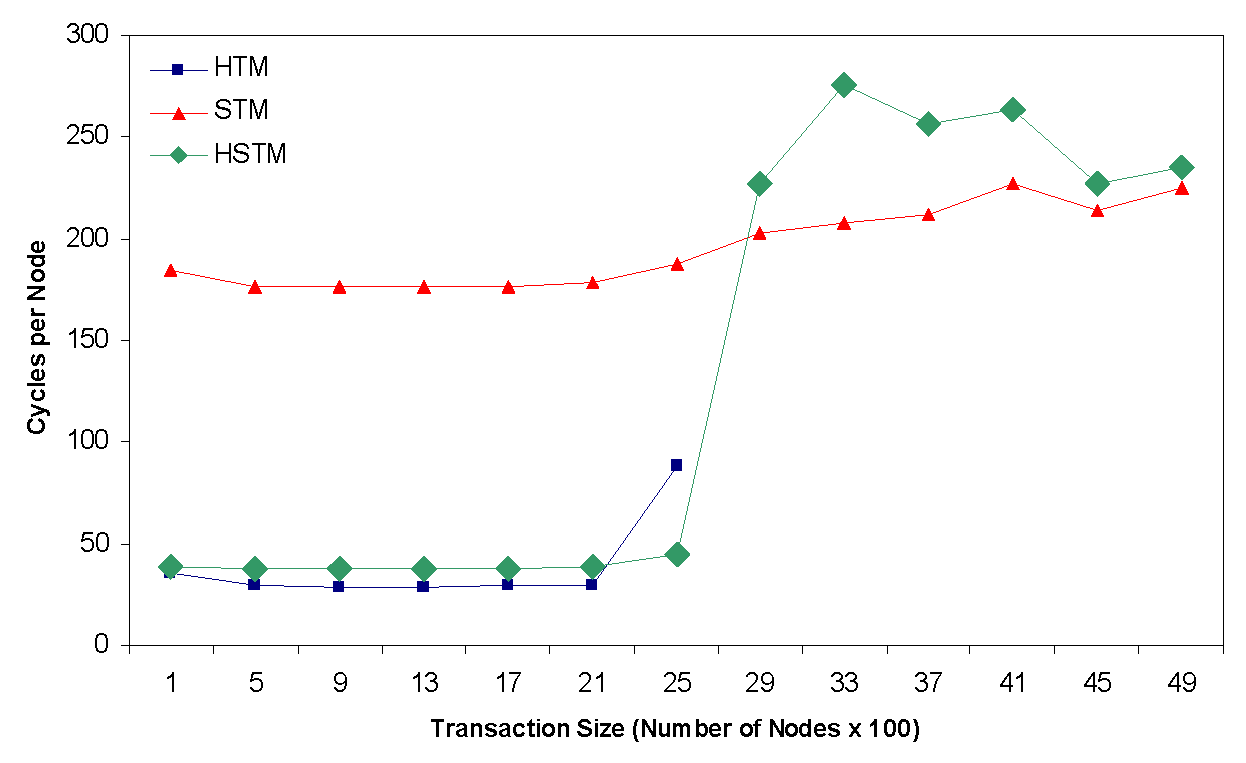
\includegraphics[width=3.25in,clip=true]{Figures/sean_lie_6b}%
\end{center}%
\caption[Hybrid performance on simple queue benchmark.]
{Performance (in cycles per node push on a simple queue
  benchmark) of LTM~\cite{AnanianAsKuLeLi04} (HTM), the
  object-based system presented in this paper (STM) and a hybrid
  scheme (HSTM).}%
\label{fig:hybrid}%
\end{figure}

We've seen that UTM and LTM can operate
with very little overhead, but hardware schemes encounter difficulties
when scaling too very large or long-lived transactions.  We have overcome
some of the difficulties with an overflow
cache (LTM), or by virtualizing transactions and dumping their
state to a data structure (UTM).  However, it is worth
considering whether this extra complexity is worthwhile: why not
combine the strengths of our object-based software transaction system
(explicit transaction state, unlimited transaction size, flexibility)
with the fast small transactions at which a hardware system naturally excels?

\figref{hybrid} presents the results of such a combination.
In the figure, combining the systems is done
in the most simple-minded way: all transactions are begun in
LTM,
and after any abort the transaction is restarted in the
object-based software system.
  The field flag mechanism described in
\secref{flagfield} ensures that software transactions properly abort
conflicting hardware transactions: when the software scribbles
\FLAG over the original field the hardware will detect the conflict.
Hardware transactions must perform
the \texttt{ReadNT} and \texttt{WriteNT} algorithms to ensure they
interact properly with concurrent software transactions, although these
checks need not be part of the hardware transaction mechanism.
In the figure, the checks were done in software, with an implementation
similar to that described in \secref{counter-bench}.

The figure shows the performance of a simple queue benchmark as the
transaction size increases.  The hardware transaction mechanism is
fastest, as one would expect, but it performance falters and then
fails at a transaction size of around 2500 nodes pushed.  At this
transaction size the hardware scheme ran out of cache; in a
more-realistic system it might also have run out of its timeslice,
aborting (LTM) or spilling (UTM) the transaction at the context
switch.

Above HTM in the figure is the performance of the software transaction
system, which is about 4x slower.  This is a pessimistic figure: no
special effort was made to tune code or otherwise minimize slowdown,
and the processor simulated had limited ability to exploit ILP (2 ALUs
and 4-instruction issue width).  However, the software scheme is unaffected by
increasing transaction size.

The hybrid scheme successfully combines the best features of both.  It
is only about 20\% slower than the basic hardware scheme, due to the
read and write barriers it much implement, but at the point where the
hardware stops working well, it smoothly crosses over to track the
performance of the software transaction system.

There are many fortuitous synergies in such an approach.  
Hardware support for small transactions may
be used to implement the software transaction implementation's
Load Linked/Store Conditional sequences, which may not
otherwise be available on a target processor.
The small transaction support can also facilitate a functional array
solution to the large object problem, as we saw in
\secref{lf-fun-arr}.  We might further improve performance by adding a
bit of hardware support for the \texttt{readNT}/\texttt{writeNT}
barriers~\cite{ClickTeWo05}.

I believe this hybrid approach is the most promising direction for
transaction implementations in the near future.  It preserves the
flexibility to investigate novel solutions to the outstanding challenges of
transactional models, which we will review in the next chapter, and
solves an important chicken-and-egg problem preventing the development
of transactional software and the deployment of transactional
hardware.  Since the speed of the hardware mechanism is tempered by
the cooperation protocol of the software transaction system,
high-efficiency software transaction mechanisms, such as the one
presented in this thesis, are the key enabler for hybrid systems.
